\chapter{Introduction}
\label{chap:Intro}

\section{Motivation}
\label{sec:motivation}
Software organizations and developers are continuously confront the needs
to improve their software processes: the software product should meet
customers' requirements better; it should have less bugs; development
process needs to be more stable and predictable; productivity should be
improved to kick the software out of door as early as possible and so on.
Unlike other disciplines such as civil engineering and mechanic
engineering, software engineering is still too young to have mature
software process and quality control process. Software is very cognitive
complicated and software development is a very creative process; thus,
each software is unique and there are no two projects that are exactly the
same. It's challenging to improve software development process.

To a software development organization there are two ways to improve its
development process: one is to identify problems in current process and
solve the problems internally; another one is to adopt successful practices
from others. Internal software process improvement program is often through
process quality control and improvement program. It is heavily emphasized
by SEI's capability maturity model (CMM) and standard ISO9001. Personal
Software Process (PSP) and Team Software Process (TSP) are two processes
proposed by SEI to achieve internal process improvement continuously.
Adopting best practices from others is another way to improve software
process by borrowing others' successful experiences. Usually it comes with
the introduction of new technologies in current development process. For
example, another development tool can be used because it has elegant
features and powerful capabilities; continuous integration can be adopted
to maintain a working version and detect problems early before they sneak
into the final product; software review can be adopted to improve software
quality by peer inspection. Of the two improvement programs, internal
process improvement is gradual and steady, while adopting external best
practice may bring dramatic changes to the development process.

Best practices are from prior successful experiences and they provide a set
of guidelines and recommendations to improve software development. Although
they proved to be successful elsewhere, they may or may not be appropriate
in a new organization. Managers in the new organizations are either
persuaded by consultants or inspired by other projects' successful stories
to exercise a new best practice. Introducing best practice is more or less
a trial-and-error approach, and normally project leaders manage and provide
supports to best practice deployment. To software developers, adopting new
best practice is passive, and they may have different opinions. Everett
Rogers modeled new technology adoption process as adoption curve
\cite{Potter:02}, in which there are five kinds of adopters when a new
technology is introduced: innovators, early adopters, early majority, late
majority and laggards.  When a new technology is introduced there is always
the learning process too.  Developers may have slow start at the beginning
before they understand the best practice well. Adding these factors
together, there will have a lot uncertainness when a new best practice is
exercised. Studying and evaluating the applicability of a new best practice
needs thorough consideration and understanding of development process. It
is fairly reasonable to conclude that the evaluation process will be more
error-prone if the practice itself is hard to be understood or it has high
discipline requirements.

Because of the nature of software development, it is expensive and
cumbersome to do qualitative empirical software best practice and process
research in software engineering. Good tools are demanded to facilitate
empirical software engineering research.

\section{State-of-art of Empirical Software Process Study}
Considering various type of data in software development Torii et al
developed Ginger2 \cite{Ginger2} system to support computer-aided empirical
software engineering. Ginger2 is an integrated environment to do \textit{in vitro} 
(laboratory) study by integrating eye-tracking system, 3D motions
and skin resistance level measurement altogether. Torii, et al 
modeled debugging process, analyzed developer's behaviors when a bug was
generated and studied collaborative debugging between two developers with 
Ginger2. It is costly to setup a Computer-Aided Empirical Software Engineering 
(CAESE) environment like Ginger2 and clearly it will distort test subject's
behaviors. The post-experiment data analysis work is massive and labor
intensive.

Cook and Wolf implemented a system called Balboa \cite{Cook:95} to discover
and validate formal software process with finite state machine. Balboa is
an event-based model of process actions and it infers a formal model from
the events of process execution. Unlike Ginger2, data collection and
process discovery are automated and they compared three methods RNet, KTail
and Markov in generating finite state machine of the process execution
with development event stream \cite{Cook:95}. They three generated
different finite state machine models to ISPW 6/7 process with some degree
of similarities. The models could be accurate to represent the real
software development process but it has too many states such that it is
extremely hard to interpret the process models and process expert's
knowledge are needed. Jensen and Scacchi automated the discovery and
modeling of open source project NetBean's development by pulling out the
web activities and interactions among developers through email, message
board and instant messaging\cite{Jensen:04}. Instead of inferring software
process blindly as Cook they used the prior knowledge of software
development to discover software process. They drew out the hyperlinked
picture of NetBeans project's requirements and release process to have
process fragments and assembled them into PML descriptions. They suggested
``a bottom-up strategy for process discovery, together with a top-down
process meta model''\cite{Jensen:04} to automate process discovery and
modeling. 

In empirical software engineering discipline, survey, experiment and case
study are three most widely used research methods. Researchers prefer to
case studies because there are too many internal and external variables to
control in the experiment. Ginger2 environment implements a complete set of
data collection tool to study development activities. Drawback of Ginger2
is that it is limited to \textit{in vitro} setting and it is impossible to
apply it on \textit{in vivo} experiment with many subjects to have
controlled experiments. The process discovery and automation sounds great
but it lacks of the in-depth knowledge of development process. It may take
tremendous amount of efforts to have the model, interpret it and find ways
to improve software process. Instead of looking for tool support in
empirical study, researchers often observation or test subjects' self
report to conduct experimentation. Perry, \textit{et al} studied time usage
in software development with both direct observation and self-reporting in
their research \cite{Perry:95}. Researchers often do Personal Software
Process (PSP) in curriculum and it is part of course requirements to submit
PSP report to ensure students do PSP in their course project development
\cite{Bullers:04,Hou:98}. M\"uller and Hagner had a case study on Test-Driven
Development in University of Karlsruhe\cite{Muller:02}. The experimentators 
asked the test subjects several times during the experiment to make sure
they did Test-Driven programming. 

The tool support is still not there yet to facilitate empirical researchers
to study phenomenon associated with software development. We are aiming to
develop a highly automatic tool to have not only in-depth knowledge of
software development process but also the evaluation of process execution
to reduce the impact of internal validity problem in empirical software
process study. Following sections covers how we designed the software
development stream analysis (SDSA) framework to serve get to this goal.

\section{Software Development Stream Analysis (SDSA)}
\label{sec:sdsa}
With my research work I introduce a bottom-up approach to derive and
evaluate best practice execution in software development automatically with
the help of Hackystat platform \cite{csdl2-02-07}. It supplies a
quantitative measure to best practice and generates reports to help
developers have more stable and disciplined software process. There is
almost no human intervention except for installing Hackystat sensors and
pulling automated generated report of best practice evaluation.

My strategy is to analyze software development microprocess with software
development stream analysis (SDSA) framework.  Microprocess is a meta unit
of software development. Developer has one task on hand only in a
microprocess and all development activities serve to accomplish this task.
We can come up with a few example to see what microprocess is.  The
development activities to fix a bug in software maintenance form a bug fix
microprocess. The procedure to implement a feature or story is a
development microprocess. In Test-Driven Development (TDD) an
red/green/refactor cycle is also a microprocess. Generically, we define
microprocess as a group of continuous activities in software development in
order to fulfill a certain task. It is up to researchers to decide what
activities account for a microprocess based on research purpose.

SDSA has four components data collection, development stream construction,
microprocess tokenization and microprocess identification.

\subsection{Data Collection}
SDSA is built on top of Hackystat so it can utilize the services provided
by Hackystat\cite{csdl2-02-07} to relieve the cumbersome data collection
overhead. It already has more than 10 sensors to collect software metrics
data from most popular development tools. In Hackystat, software metrics
are automatically collected by attaching sensors to development tools,
metric data are sent to a dedicated server for data storage and analysis.
SDSA is a web-based system to analyze sensor data collected by Hackystat
to inspect software execution process. 

\subsection{Development Stream Construction}
Hackystat sensors collect development activities, object-oriented metrics,
unit test invocation, compilation, commits and so on and stores these data
in Hackystat server. We reduce sensor data into development activities,
continuous activities make of development stream in SDSA framework.
Development stream is a collection of all development activities over a
period.  Table \ref{tab:stackstream} is part of the software development
stream whilst I worked on a stack data structure implementation.
\begin{table}[!h]
\centering
  \begin{tabular}{|llll|}
  \hline
    23:43:57 & TestStack.java & ADD CLASS & package org.sci \\
    23:43:57 & TestStack.java & ADD IMPORT & import junit.framework.TestCase \\
    23:43:57 & TestStack.java & MOVE CLASS & org.sci --\textgreater TestStack.java \\
    23:44:19 & TestStack.java & ADD METHOD & void testEmptyStack() \\
    23:44:38 & TestStack.java & TEST EDIT & 6sec \\
    23:44:39 & TestStack.java & COMPILE & Stack cannot be resolved \\
    23:45:07 & Stack.java     & ADD CLASS & Stack.java \\
    23:45:07 & Stack.java     & BUFFTRANS & FROM TestStack.java \\
    23:45:34 & Stack.java     & ADD METHOD & Stack() \\
    23:45:56 & Stack.java     & PRODUCTION EDIT & 18sec \\
    23:46:02 & TestStack.java & BUFFTRANS FROM & Stack.java \\
  \hline
  \end{tabular}
  \caption{Development Stream of Stack Implementation}\label{tab:stackstream}  
\end{table}
Stack works on the principle of Last-In-Last-Out(LILO). This development
depicts how I implemented stack with best practice Test-Driven Development
(TDD). I started it with the creation of test class
\textsf{\textbf{TestStack.java}} to drive the implementation of stack. Test
case \textsf{\textbf{void testEmptyStack()}} is added right after because
it is an easy task to test and implement. The test class can not compile
because object \textsf{\textbf{Stack}} does not exist yet. Then I went
ahead to implement stack object to solve the compilation error.  The
development stream empowers us to retrospectively play back detailed
development process.

\subsection{Microprocess Tokenization}
Development stream has rich information on software process. It's easy to
analyze a small portion of the development stream, but it is not feasible
to look up the entire development stream with thousands of development
activities. And it might not be necessary to analyze tons of activities as
Cook \cite{Cook:95} and Jensen \cite{Jensen:04} in their researches.
Nowadays, software development is incremental and iterative, we can study
the development process iteration by iteration without bother to look up
massive amount of data. We name this iterative development process as
microprocess in which there are only limited number of development
activities.

In software development, developers always have processes or best practices
to follow on.  They define a set of rules and recommendations to regulate
software development. Software best practice either defines the order of
development activities or adds new tool support to software development.
For example, incremental build is the best practice to audit program's
change and build system once there are changes to reduce compilation
failures; unit test best practice emphasizes that developers should write
their unit tests to improve the quality of programs instead of relying on
quality assurance help at the later stage in the software development
life-cycle. In incremental and iterative software processes, software best
practices are repetitive.  By separating development stream into iterations
we will be able to demonstrate and examine the best practice deployment in
each iteration. An iteration is also a microprocess and the separation 
method is called microprocess tokenization. Tokenizers need to be carefully
designed to chop development stream into meaningful chunks.

\subsection{Microprocess Identification and Evaluation}
A microprocess will contain a series of activities with information about
best practice execution. We chose rule-based system to identify and evaluate
execution of best practice in a microprocess. In rule-based system
knowledge is represented in the form of \textit{if...then...}
rules\cite{Luger:02}. Inference engine in rule-based system can apply best
practice rules and recommendation on microprocess activities to look for
matched patterns and problems. Figure \ref{fig:concept} is the conceptual 
model.
\begin{figure}[h]
  \centering
  \includegraphics{figs/ConceptStructure.eps}
  \caption{Microprocess Identification and Evaluation}\label{fig:concept}
\end{figure} 

Software Development Stream Analysis (SDSA) framework unites data
collection, development stream construction, microprocess tokenization and
microprocess identification and evaluation together to sustain empirical
software process study. In my thesis work I will apply it on Test-Driven
Development (TDD), one of the most popular and well-practiced best practice
among 12 Extreme Programming (XP) practices. I chose TDD as the starting point
to exercise SDSA paradigm on empirical software process research because of
the following reasons: 
\begin{itemize}
\item {TDD is a disciplined practice;}
\item {TDD is iterative and has two simple rules only;}
\item {Research conclusions of TDD are not inclusive;}
\item {Professional software developers embrace TDD.}
\end{itemize}

\section{Test-Driven Development}
\subsection{What is Test-Driven Development}
Test-Driven Development was first coined by Beck and his colleagues when
they developed Chrysler C3 project, a payroll system in SmallTalk. In C3
project, they started a new practice to implement component test first and
developed it as Test-First Programming, the precedence of Test-Driven
Development. Some people prefer to calling it Test-First Design (TFD)
because they think TDD is more about design than programming. With TDD
developers \textit{(1) write new code only if an automated test has failed;
  (2) eliminate duplication} iteratively in software
development\cite{Beck:03}.

New code is added only when there is a failed unit test and TDD is to
create ``clean code that works''\cite{Beck:03}. TDD development process is
a stop-light pattern, a TDD cycle starts with failed unit test in red
light, and it turns green after the code is implemented to make unit tests
pass. TDD philosophy ``clean code that works" means that developer writes
only enough code to make unit test pass without committing too much work.
The suite of unit tests gives developer confidence and courage to refactor
the implementation code afterward to eliminate the duplication
\cite{Beck:03}.

\subsection{Widespread of Test-Driven Development}
People often use ``test infected"
\cite{TestInfected,ObjectMentorTDD,MasonBlog,EichertBlog} to describe
developer who sticks to TDD after seriously practices it. The code will be
100\% tested because all of the code are driven by unit tests. Their
existence makes developers feel free to refactor code constantly in the
development process. TDD is getting popular in software industry and some
organizations even demand all developers stick to TDD.  The extension of
xUnit framework on programming languages and development of mock testing
technique make it feasible to test almost everything, which helps to boost
the acceptance of TDD.

Test-Driven Development has its own site at http://www.testdriven.com and
user group powered by Yahoo\cite{TddYahooGroup}.  It is a platform for TDD
developers to share information, exchange ideas and announce supporting
tool releases \cite{TestDrivenWeb}. A couple of books
\cite{Beck:03,Astels:03,Link:03,Andy&Dave:03} were published to disseminate
testing and Test-Driven Development, and some consulting companies provide
TDD
training\cite{AdaptionTddWorkshop,IndustrialLogicTddWorkshop,BENUGWorkshop:04,ClarkwareWorkshop:04,OsheroveWorkshop:04}
to improve TDD practice in software industry.

\subsection{Test-Driven Development Research}
George and Williams ran through a structured experiment to compare TDD
group and control group who developed in waterfall-like process
\cite{George:03}. The research found that TDD group yields superior
external code quality compared to waterfall-like controlled group, although
TDD group took 16\% more time on development. Majority TDD developers
thought that TDD is effective and improves programmers' productivity
(80\% and 78\% respectively). In the mean time all developers were assigned
as pairs randomly in the experiment, which makes it significantly different
from other case studies. Researches in pair-programming indicates that
pair-programming has social impacts on developers' behaviors because of
pair pressure. Maximilien and Williams conducted another vertical
experiment at IBM without pair-programming \cite{Maximilien:03}. They found
that the new system reduced defect density by 50\% in functional
verification test(FVT) compared to the legacy system that was developed in
ad-hoc manner. There was somewhat productivity decrease in the experiment
but developers inclined to continue using TDD in future software
development.

Geras et al. designed an experiment to ask participants work on two projects
with Test-First and Test-Last in different order in two groups
\cite{Geras:04}. There are only slightly differences on effort, tests per
KLOC, customer test invocations and unplanned failures after delivery
between Test-First and Test-Last processes. In the experiment developers
worked on their own following the script without management and some of
them even failed to submit the working program. M\"uller and Hagner had a
similar case study in University of Karlsruhe\cite{Muller:02}. The TDD
group and controlled group worked on a same graphic library and they
verbally confirmed that Test-First subjects got along with Test-First
process. They concluded that TDD does not accelerate the implementation and
the resulting programs are not more reliable except that it supports
better program understanding. 

These case studies give Test-Driven Development a shot and compare it
against traditional ad-hoc or waterfall process. The conclusions are
variant rather than unanimous. Researches realized that Test-Driven
Development has high discipline requirement and used pair-programming,
management, script guideline or verbal confirmation in the experiments.
These measures are helpful in removing internal validity problem but the
development processes are not measurable and controllable, which may
attribute to the differences on divergent conclusions on TDD. It is still
challenging to adopt TDD \cite{Janzen:05} so we do not know how test
subjects conducted software implementation differently in the studies.
Florac \cite{Florac:99} explained that software process can be measured and
improved with statistics process control (SPC). My work is to improve the
quality of empirical study on best practice and TDD specifically.

\subsection{Test-Driven Development Microprocess Identification and Evaluation}
As I discussed in section \ref{sec:sdsa}, Test-Driven Development is a good
fit to Software Development Stream Analysis (SDSA) framework. In this
section I am going to address issues that are connected with TDD.

\subsubsection{Data Collection}
In TDD, developer works on test code and production code interchangeablly
in an iteration, test is executed frequently to guide code implementation
and guard code refactoring.  Essential data to be included are
\begin{itemize}
\item {Test invocation and its result}
\item {Test code implement}
\item {Production code implementation}
\item {Refactoring}
\end{itemize}
Compilation error can also be collected to inspect microprocess in small step
with compilation failure on test code caused by missing production code.
Commit activity data is a plus when version control system is employed.

\subsubsection{Test-Driven Development Stream}
The SDSA framework need to be plugable so that we can just plug in the
interesting activities into the development stream. To Test-Driven
Development, we will include unit test substream, edit (on documentation,
unit test and production code) substream, refactoring substream and
compilation substream, and commit substream if applicable.

\subsubsection{Test-Driven Development Microprocess Tokenization}
Test-Driven Development is in stoplight pattern. It implies that a
microprocess ends with successful unit test execution, which is green like
traffic light to mean that the software system is under controlled and
there is no failing tests. The green light marks the end of one microprocess
so we can design \textit{Test-pass} tokenizer to tokenize TDD development
stream. Figure \ref{fig:TddMicro} is a TDD microprocess example.
\begin{figure}[h]
  \centering
  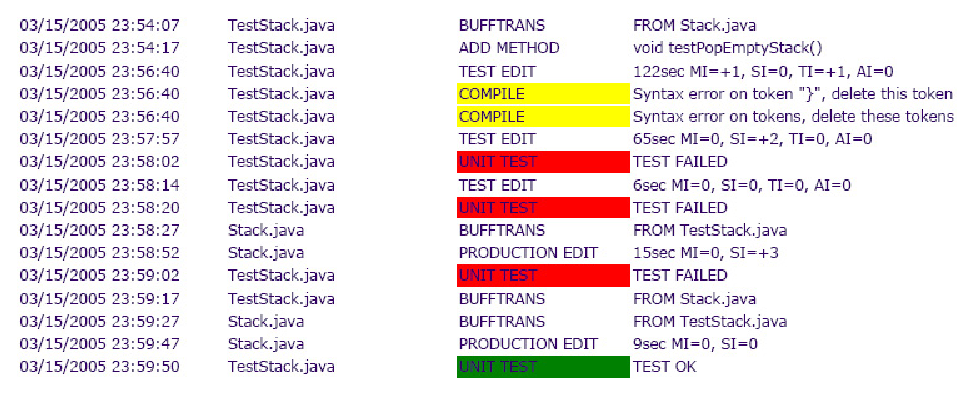
\includegraphics[width=0.9\textwidth]{figs/TestPassEpisode.eps}
  \caption{A TDD Microprocess Example}\label{fig:TddMicro}
\end{figure} 

\begin{comment}
Technically test-pass tokenizer is enough to detect iterations of
Test-Driven Development. However, in team software development, developers
also deploy their work with the whole system to make sure new code will not
break it before integration. To accommodate team software development we
defined \textit{Commit} and \textit{Command} tokenizers for integration and
deployment activities. On the other side, developers may not do TDD or
occasionally step away from TDD without frequent unit test invocations. We
defined \textit{Buffer Transition} tokenizer to divide this kind of
micro-processes into smaller buffer transition micro-processes for further
analysis.

\begin{itemize}
\item \textit{Commit tokenizer} ends an episode when it encounters a bunch
  of file commit activities. It can be used to inspect what developers do
  before integration.
\item \textit{Command tokenizer} ends an episode when there are some
  consecutive command build activities to deploy system in local
  environment.
\item \textit{Test Pass tokenizer} ends an episode when there are
  successful unit test invocations. We implemented it to find the iterations
  in Test-Driven Development.
\item \textit{Buffer Transition tokenizer} starts an episode when it
  encounters consecutive buffer transition activities. It sums what
  developers did to the working buffer.
\end{itemize}
\end{comment}

\subsubsection{TDD Microprocess Identification and Evaluation}
Test-pass tokenizer partitions development stream into many iterations that
end up with successful unit test execution. In term of TDD, a test-pass
episode can be either ``test-driven'' or ``refactoring''. The significant
property of refactoring is that there is no new test case in refactoring 
episode. With this character we can classify test-pass episodes of TDD into 
two categories, ``test-driven'' and ``refactoring''.  Moreover, a test-pass 
episode with test creation may or may not be ``test-driven''.  Test-Driven 
Development implies the order of development is to ``test a little, code a 
little and repeat."\cite{Beck:03} such that it will be ``test-last'' if test 
is not created before code implementation. Figures \ref{fig:tdd} and
\ref{fig:refactoring} illustrate different kinds of ``test-driven'' and 
``refactoring'' episodes respectively.

\begin{figure}[h] 
  \centering
  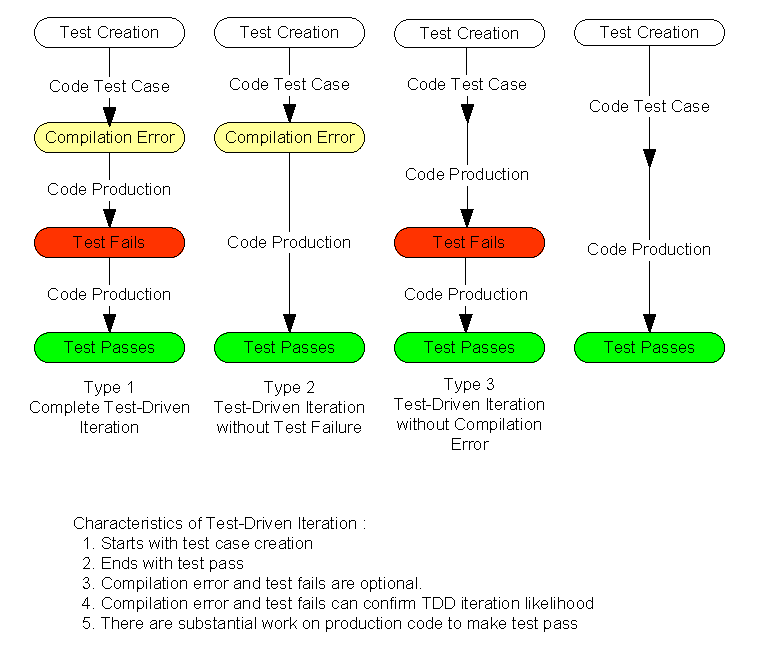
\includegraphics[width=0.8\textwidth]{figs/TDD.eps}
  \caption{Test-Driven Episode Classification}\label{fig:tdd}
\end{figure} 

\pagebreak
\begin{figure}[h] 
  \centering
  \includegraphics[width=0.8\textwidth]{figs/Refactoring.eps}
  \caption{Refactoring Microprocess Classification}\label{fig:refactoring}
\end{figure} 

\section{Research Statement}
Software engineering is an empirical discipline and best practice is a very
important component in this field. Lacking of good tool support greatly
impacts validity of the research conclusions. My research is to design and
develop a paradigm to facilitate empirical software research on iterative
software processes and best practices effectively by the introduction of
software development stream analysis (SDSA) framwork. I am going to study
how this framework can support Test-Driven Development empirical study in
my thesis work and the weakness of this automation approach. Upon success
this research will power empirical researchers both qualitative evaluation
and quantitative measure of software best practice executions.

\section{Research Methods}

\section{Roadmap}
This thesis work is to evaluate best practice execution in software development 
with development stream. Chapter \ref{chap:relatedwork} is the related
literature work on Hackystat, software process automation, event stream and
Test-Driven Development. The system design structure and implementation details
are described in chapter \ref{chap:implementation}. The framework is tested
against Test-Driven Development with a series of experiments in 
chapter \ref{chap:evaluation}.
\begin{comment}

 as in Figure \ref{fig:EpisodeTree}.
\begin{figure}[htbp] 
  \centering
  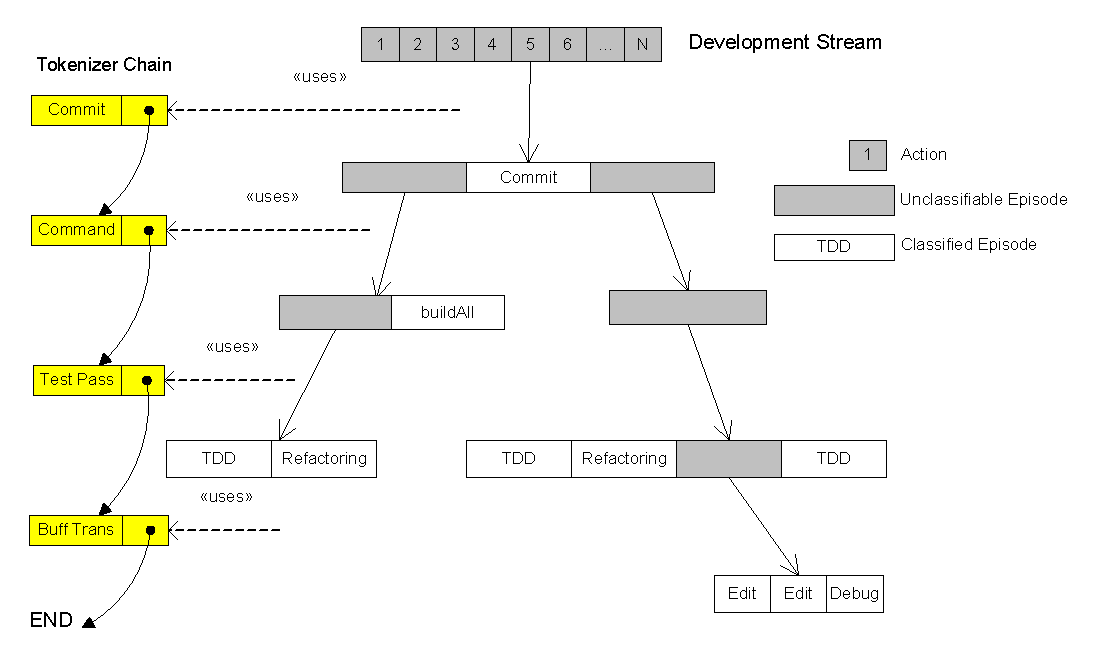
\includegraphics[width=0.8\textwidth]{figs/EpisodeTree.eps}
  \caption{Episode Tree}\label{fig:EpisodeTree}
\end{figure} 

Some empirical case studies \cite{George:03}, \cite{Maximilien:03}
reported successes on TDD practice. According to these studies TDD group
passed more black box tests than TLD group and they spent less time on
projects than TLD group. Even though most empirical studies drew positive
conclusion on Test-Driven Development there are still some neutral or
negative reports on TDD. Geras etc. \cite{Geras:04} found that there is
little or no difference in developer productivity in TDD and TLD processes.
Another study \cite{Muller:02} concluded that TDD does not accelerate the
implementation and the resulting programs are not more reliable than TLD.

\section{Validation}
Unlike many other cumbersome software processes such as Spiral model, PSP or
RUP Test-Driven Development is very lightweight. It contains two simple
rules only. In practice TDD is hard to follow compared to other processes
because there is no management involved in the development. In situations
that pair programming is not involved developers are fully responsible for
TDD execution by themselves without monitoring. This weakness will bring
many questions to TDD process. Do developers do Test-Driven Development
when they are told to do so? And if they do how well they do TDD in their
development? Do developers always follow two TDD rules?

In my thesis study I will build a system on top of Hackystat to answer
these questions as well as provide a tool to discipline TDD process.  There
are two goals to pursue in my work. One is to study how the development is
being done, especially how the unit testing is conducted in Test-Driven
Development. Another goal is to study properties of TDD. Will developers
spend more time on development and yield high quality code or not? Will the
test coverage be naturally 100\%?

Scott Ambler's UML diagram (Figure \ref{fig:TDDSteps}) depicts TDD development
iterations.

\begin{figure}[htbp] 
  \centering
  \includegraphics{figs/TDDSteps.eps}
  \caption{The Steps of TDD}\label{fig:TDDSteps}
\end{figure} 

\begin{itemize}
\item The first step is to add a test quickly. Basically it just fails the
  code.
\item Next run your test or test suite to make sure the new test does fail.
\item Make changes to the function code to make test pass. As long as it
  can make test pass you even can fake the implementation, for instance,
  return a constant number.
\item Run your tests again. If it still fails you go ahead to update your
  function code. Once all tests pass you can start over with a new test.
\end{itemize}



 
In the early era of software development there is no software process.
Software systems are developed in a chaotic style and their successes
depended largely on individual's skills and capabilities. Water-fall model
is the first and most popular software development process and it still
exists in many organizations. In water-fall model software development is
divided into stages from requirement analysis to operation and testing is
conducted after project is implemented. Bugs and defects found in testing
will be fed back to the development team or maintenance team. Since bugs
and defects are revealed at the late stage of software development
water-fall model is reluctant to meet customer's requirements and defect
fix. If defects are rooted from design it will be extremely hard to adapt
changes according to water-fall model.

Modern iterative incremental development(IID) was developed to fix this
problem by dividing a large project into many parts.  They are implemented
iteratively. Each iteration can be a mini-waterfall process so that defects
can be fixed and changes can be made very quickly.  Spiral model is the
first process definition to formulate iterative incremental development
practice. Other variations like prototyping, RAD, CleanRoom, Scrum, RUP,
FDD, Extreme Programming are used in many projects successfully.  Latest
development of continuous integration builds system once a day. In these
processes testing is done after some amount of work is finished to improve
project quality.
  
\section{Personal Software Process}
\label{sec:psp}

   Introduce LEAP and Hackystat.

\section{Test-Driven Development}
\label{sec:tdd}

\subsection{Unit Testing}
\label{sec:UnitTest}
Object-oriented technique treats abstract concepts as entities such that
each of them is independent and can exist without relying on other code.
Unit testing was invented to test a component before it is integrated to
interact with other components. Unit testing originates from
pre-object-oriented era and an individual test concentrates on a single
unit of the system rather than on the entire system. At present when we say
unit testing it refers to component testing. In object-oriented world a
component test usually tests an object or class which is the smallest component
of a system. ``In computer programming, a unit test is a method of testing the
correctness of a particular module of source code.'' \cite{UnitTestWiki}

Unit testing is becoming more and more popular in modern software
development.  The de facto unit testing standard, ``xUnit'' framework, is
already ported to more than 30 language support. It makes test automation
be feasible and test cases created with XUnit framework can server as
regression test suite too. Except for verifying correctness of each class
unit testing is also the executing documentation. In recent software
project development unit testing is integrated into development process in
many organizations. Test cases are written by developers who are also
responsible for programs. Even though source code is visible to developers
but unit testing is still thought as black-box testing because it simulates
calls from other components.  

JUnit is the most well-known XUnit framework implementation in software
development and other dialects NUnit, CPPUnit, PyUnit so on and so forth
are created to make writing unit tests be very simple in different
programming languages. JUnit and NUnit also have IDE plug-in supports so
that a unit test case can be exercised by just a single click. For
continuous integration unit test cases can also be batched together to run
as ANT task. Since writing unit tests is not a cumbersome job any more it
is recommended to write unit tests in the development process instead of
allocating extra resource to let quality assurance testers to create unit
tests separately. It improves the effectiveness of testing such that
software systems are in high quality before they are delivered to quality
assurance department or customers if there is no quality assurance process.
Since less time is needed to do quality assurance it will save overall
development time conceptually.


In TDD unit testing is crucial because it drives the implementation and provides
instant feedback of the developing code to the developers. The XUnit
framework family make it easy to write tests and execute tests often in
software development.

\section{Thesis Work}


\section{Road Map}

\end{comment}
\begin{comment}
\label{sec:ResearchObjective}
Test-Driven Development is being accepted by more and more developers and
organizations. On the other side there are still many developers and
researchers resist Test-Driven Development or doubt its effectiveness in
software development. Kent Beck argued that TDD will not increase
development cost but can actually improve productivity as well as software
quality. Ron Jeffries's pithy word ``Clean code that works'' is the goal
of Test-Driven Development.


\section{Extreme Programming(XP) and Test-Driven Development(TDD)}
[How good is unit test? and why TDD]

  
This testing pyramid corresponds to software system development process.
In general a large system is divided into many components to be implemented
independently. Unit testing is created to verify correctness of each
component before it is integrated into the system.
  
Usually unit testing is done by programmers themselves to verify the
correctness or by quality assurance specialists to find errors in the
existing code.  According to the cost model of removing bugs in different
software development stages removing bugs in development phase is the most
cost-effective way.  Because unit testing is good from many aspects Extreme
Programming, an agile software development process, advocates Test-Driven
Development (TDD) as its core component. In TDD unit tests are
incrementally written prior to code implementation \cite{George:03} thus
it drives software specification design in addition to validating and
verifying program correctness. Because of this capability TDD is also
called Test-First Design (TFD). As comparison the old way writing unit
tests after code is ready is called Test-Last Development(TLD).
  
  
  The controversial conclusions can be either from TDD process itself or
  from the poorly executed experiments. There is one thing in common that
  all these studies failed to address how they managed experiments to
  guarantee TDD developers do Test-Driven Development while TLD developers
  do Test-Last Development in their studies. There is no process data
  available to crossly validate process disciplines. The lack of
  fine-grained process data and software metrics makes it impossible to
  conclude whether developers were doing TFD, ad-hoc or TLD in the previous
  experiments; thus, conclusions drawn from these experiments are weakened
  and become questionable. In my thesis I will add in-process metric
  support provided by Hackystat to study how unit tests are created and
  exercised in the development process to regulate software development.
\end{comment}

\begin{comment}  
\section{Testing}
\label{sec:Testing}
Testing is very important to software project success because developers
can not always produce perfect code that works well at the first time. Many
reasons determine that we need testing in software development. First of
all, many software systems deal with large number of states with complex
algorithms, also it is hard and impossible to address all system
requirements at the beginning of software projects development. Developers
always have to deal with new and changing requirements during the
development.  Another important factor is that software projects are
written by developers.  As human beings developers are not good at
repeative programming work without committing mistakes.  Since software
development is error-prone many design and development support tools such
as flowchart, dash board, UML , compilers, debuggers, version control
system, project management software, bug tracking system and software
review etc are brought up to support qualitative software development.
Moreover, there are rare software projects developed and maintained by an
individual programmer nowadays. The ineffective collaboration and
cooperation in the developing team will make software volatile to defects
and bugs too \cite{Pfleeger:01}.  To ensure software quality there are
quality assurance departments in many software institutes and many testing
techniques appeared in the development of software engineering discipline.
From visibility of source code there are white-box testing and black-box
testing. Depending on when testing happens there are unit testing,
regression testing, integration testing, system testing and acceptance
testing which can be done by programmers, quality assurance testers or
customers manually or automatically.

\begin{figure}[ht] 
  \centering
  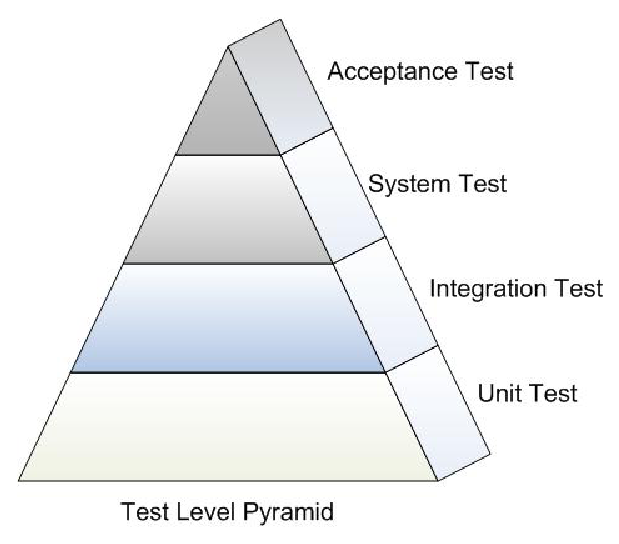
\includegraphics[width=0.5\textwidth]{figs/TestLayerPyramid.eps}
  \caption{Software Testing Pyramid}\label{fig:TestLayer}
\end{figure} 

In tradition, software testing is thought as quality assurance testers' or
customers' job in water-fall software process model. Even in recent
iterative incremental development (IID) models quality assurance
specialties and customers still play important roles on testing.


\section{Software Processes}
\label{sec:SoftwareProcess}
In the early era of software development there is no software process.
Software systems are developed in a chaotic style and their successes
depended largely on individual's skills and capabilities. Water-fall model
is the first and most popular software development process and it still
exists in many organizations. In water-fall model software development is
divided into stages from requirement analysis to operation and testing is
conducted after project is implemented. Bugs and defects found in testing
will be fed back to the development team or maintenance team. Since bugs
and defects are revealed at the late stage of software development
water-fall model is reluctant to meet customer's requirements and defect
fix. If defects are rooted from design it will be extremely hard to adapt
changes according to water-fall model.

Modern iterative incremental development(IID) was developed to fix this
problem by dividing a large project into many parts.  They are implemented
iteratively. Each iteration can be a mini-waterfall process so that defects
can be fixed and changes can be made very quickly.  Spiral model is the
first process definition to formulate iterative incremental development
practice. Other variations like prototyping, RAD, CleanRoom, Scrum, RUP,
FDD, Extreme Programming are used in many projects successfully.  Latest
development of continuous integration builds system once a day. In these
processes testing is done after some amount of work is finished to improve
project quality.



\section{Extreme Programming}
\label{sec:XP}
Extreme programming (XP) grows very fast recently and many organizations
are using it or considering to adopt it in their developments. Extreme
Programming is also one kind of iterative incremental development (IID)
process.  It begins with collecting ``user stories'', which are brief
description of tasks to be accomplished. Developers can discuss with on-site
customers to make release plan based on user stories. After each release
customer can test the sub system and give feedback to developers quickly.
XP can not only meet customers' changing requirements well but also provide
high quality code because it stresses heavily on unit tests in the
development. Four rules are enforced in extreme programming.

\begin{itemize}
\item All code must have unit tests.
\item All code must pass all unit tests before it can be released.
\item When a bug is found tests are created.
\item Acceptance tests are run often and the score is published.
\end{itemize}

To enact these rules XP projects should be developed in Test-Driven
Development process, in which unit tests are created before code
implementation.  Developers write unit tests based on user stories first
and then generate code to make test pass.
\end{comment}
